\chapter{Projeto de Estudo de Caso}
\label{chap:proj-est-caso}

%TODO ESCREVER BREVE INTRODUCAO DO CAPITULO 

Este capítulo apresenta o protocolo do estudo de caso a ser realizado. A sua definição e os requisitos necessários para sua execução são identificados e explicados. 

% Ao final um cronograma com as estimativas de tempo será apresentado.

% @Definição
\section{Definição}\label{sec:Definição}

Um estudo de caso consiste no estudo profundo e exaustivo de um ou poucos objetos, de maneira que permita seu amplo e detalhado conhecimento \cite{gil-estudo}, assim representa uma maneira de se investigar um tópico empírico seguindo-se um conjunto de procedimentos pré-especificados \cite{yin2001estudo}. 
 Uma vantagem dos estudos de caso é que eles são mais fáceis de planejar e são mais realistas, mas as desvantagens são que os resultados são difíceis de generalizar e mais difícil de interpretar , ou seja, é possível mostrar os efeitos de uma situação típica, mas requer mais análise para que se possa generalizar a outras situações \cite{wohlin_experimentation_2012}.

% Um estudo de caso tem a vantagem de prover respostas que vão além das questões de ``O que''

% @Commentario
\begin{comment}

Case studies are very suitable for industrial evaluation of software engineering methods and tools because they can avoid scale-up problems. The difference between case studies and experiments is that experiments sample over the variables that are being manipulated, while case studies select from the variables representing the typical situation. An advantage of case studies is that they are easier to plan and are more realistic, but the disadvantages are that the results are difficult to generalize and harder to interpret, i.e. it is possible to show the effects in a typical situation, but it requires more analysis to generalize to other situations 

\end{comment}

A estrutura do protocolo de estudo de caso prosposta se baseia em \citeonline{case-study-template-2008} e se apresenta dividido nos seguintes tópicos, cada um com seu objetivo específico:

\begin{easylist}[itemize]

& \textbf{Background - Seção \ref{sec:Background}}: Identificar outras estudos acerca do tópico, define a questão de pesquisa principal e suas proposições  derivadas  que serão abordado por este estudo.

& \textbf{Design - Seção \ref{sec:Design}}: Identificar se é um caso único ou múltiplo e seu propósito geral.

& \textbf{Seleção - Seção \ref{sec:Seleção}}: Critérios para a seleção do caso e descriçao do objeto de estudo.

& \textbf{Fonte e Método de Coleta de Dados - Seção \ref{sec:Fonte e Método de Coleta de Dados}}: Identificar os dados que serão coletados, definindo um plano para a coleta e como a informação será armazenada.

& \textbf{Análise - Seção \ref{sec:Análise}}: Identificar os critérios para interpretação dos resultados do estudo de caso, relacionar os dados com a questão de pesquisa e elaborar a explicação do encontrado.

& \textbf{Validade - Seção \ref{sec:Validade}}: Se baseia nos tipos de validades aplicáveis a um estudo de caso por \citeonline{yin2001estudo}, sendo elas: constructo, interna, externa e confiabiliade.

% & \textbf{Cronograma - Seção \ref{sec:Cronograma}}: Cronograma com as estimativas de tempo para as grandes estapas: planejamento, coleta de dados, análise, relatórios.

\end{easylist}

% @Background
\section{Background}\label{sec:Background}
    

\subsection{Outros Trabalhos}
% @todo melhorar
O uso do monitoramento de métricas de código-fonte num ambiente de data warehousing foi proposto e desenvolvido no trabalho de \citeonline{rego_monitoramento_2014}.

\subsection{Questão de Pesquisa}
A questão de pesquisa deriva do problema identificado, e busca definir o propósito da medição, o objeto que será medido, a questão a se tratar, e o ponto de vista que se delimita a questao \cite{Basili96b}.

Para responder a questão de pesquisa foi construído um GQM (\textit{Goal-Question-Metric}) \cite{Basili96b} representado na Figura \ref{fig:estrut-est-caso}. O GQM possui objetivos específicos para a questão de pesquisa, cada um tem suas questão específicas que busca responder com a coleta de métricas a questão maior de pesquisa e assim atender o problema do estudo de caso. 


% @Figure GQM
\begin{figure}[h!]
\centering
\includegraphics[keepaspectratio=false,scale=0.53]{figuras/figuras_pedro/estrut-estudo-caso.eps}
\caption{Estrutura do Estudo de Caso}
\label{fig:estrut-est-caso}
\end{figure}
\FloatBarrier

% \textbf{Questão de Pesquisa: \textit{A solução de data warehousing é eficaz e eficiente no monitoramento de métricas de código-fonte para o apoio à decisões de refatoração do ponto de vista da equipe de qualidade?}}

O problema se refere ao problema de pesquisa identificado. A questão de pesquisa se refere a questão geral de pesquisa. Assim foi definido um objetivo para a questão de pesquisa, e para ele foram levantadas nove questôes. A caracterização de cada item está a seguir.

\textbf{Questão de Pesquisa: \textit{O uso de um ambiente de Data Warehousing para aferição e monitoramento da qualidade interna do código-fonte é eficaz e eficiente do ponto de vista da equipe de qualidade?}}

\textbf{Objetivo 01:} Avaliar a eficácia e eficiência da solução de \textit{Data Warehousing} do ponto de vista da <equipe de qualidede> no contexto de desenvolvimento de software. \newline


\textbf{Questão 01:} Quantas tomadas de decisão foram realizadas pela equipe baseado no uso da solução?

\textbf{Fonte:} Observação em campo.

\textbf{Métrica:} número de decisões tomadas. \newline

\textbf{Questão 02:} Quantas tomadas de decisão foram realizadas pela equipe baseado no uso da solução em um <período de tempo>?

\textbf{Fonte:} Observação em campo (áudio/vídeo).

\textbf{Métrica:} número de decisões tomadas/tempo. \newline


\textbf{Questão 03:} Qual a avaliação da equipe de qualidade quanto a detecção de cenarios de limpeza de codigo?

\textbf{Fonte:} Questionário com a equipe de qualidade.

\textbf{Métrica:} muito bom, bom, regular, ruim, muito ruim. \newline


\textbf{Questão 04:} Com que frequência a equipe de qualidade encontra falhas relacionados à utilização da ferramenta?

\textbf{Fonte:} Observação em campo (áudio/vídeo).

\textbf{Métrica:} quantidade de falhas. \newline


\textbf{Questão 05:} Com que frequência a equipe de qualidade encontra falhas relacionados à utilização da ferramenta por tempo?

\textbf{Fonte:} Registro de Observação em campo (áudio/vídeo).

\textbf{Métrica:} quantidade de falhas / tempo. 

\textbf{Interpretação do valor da métrica:} Quanto mais próximo de zero melhor. X >= 0. \newline


\textbf{Questão 06:} Qual a proporção de uso da ferramenta para a tomada de decisões?

\textbf{Fonte:} Questionário com a equipe de qualidade.

\textbf{Métrica:} número de decisões tomadas / número de vezes que a solução foi usada 



\textbf{Questão 07:} Qual a quantidade de cenários que foram corrigidos após utilização da solução?

\textbf{Fonte:} Código fonte.

\textbf{Métrica:} números de cenários corrigidos por release / número de cenários encontrados por release. \newline



\textbf{Questão 08:} Qual o nível de satisfação do uso da solucão em comparação à solução anterior?

\textbf{Fonte:} Equipe de Qualidade.

\textbf{Métrica:} muito satisfeito, satisfeito, neutro, insatisfeito, muito insatisfeito. \newline


\textbf{Questão 09:} Qual a taxa de oportunidade de melhoria de código da solução em uma <intervalo de tempo (sprint, release)>?

\textbf{Fonte:} Código-fonte.

\textbf{Métrica:}  A Taxa de Aproveitamento de Oportunidades de Melhoria de Código, em uma release, é calculada como: $$ T_r =   \frac{{\sum_{i=1}^{n}{Ce_i}}}{\sum_{i=1}^{n}{Cl_i}} $$

onde $ Ce $ é o total de cenários de limpezas identificados e $ Cl $ é total de classes em uma release.

\textbf{Interpretação do valor da métrica:} 
\begin{easylist}[itemize]   
    & \textbf{Número de classes crescente e constante, número de oportunidade de melhoria estável:} Projeto cresceu mais dos que o cenários, cenários podem ou não estar sendo tratados.
    & \textbf{Número de classes crescente e constante, número de oportunidade de melhoria crescendo:} Projeto cresce junto com cenários que não são tratados com eficiência ou não são tratados
    & \textbf{Número de classes crescente ou não, mas constante, número de oportunidade de melhoria diminuindo:} Projeto cresce e cenários são tratados com eficiência.  
\end{easylist}  

% @Design
\section{Design}\label{sec:Design}

\citeonline{stake_art_1995} Identifica três modalidades de estudo de caso: intríseco, instrumental e coletivo. Dentre essas definições, este estudo de caso se caracteriza com instrumental, pois se busca um entendimento geral sobre o problema de pesquisa a partir do estudo de um caso particular. Tal característica se assemelha ao tipo de estudo de caso definido como exploratório por \citeonline{yin2001estudo}, onde a visão acurada de um caso particular poderá fornecer uma visão geral do problema considerado.

A justificativa para este estudo de um caso particular se dá pelo motivo de que o tema abordado foi pouco explorado até o momento. Assim espera-se que este caso único componha um estudo de múltiplos casos, pois segundo \citeonline{gil-estudo} esta abordagem possa inserir as evidências coletadas aqui em diferentes contextos, com o intuito de elaborar uma pesquisa de melhor qualidade.



% @Seleção
\section{Seleção}\label{sec:Seleção}

A organização selecionada para este estudo de caso foi o 
TCU.
O software que terá seu código-fonte analisado foi desenvolvido segundo a metodologia
% metodologia
, com uma equipe de 
% equipe
.

% @Fonte e Método de Coleta de Dados
\section{Fonte e Método de Coleta de Dados}\label{sec:Fonte e Método de Coleta de Dados}

Os dados serão coletados no órgão por meio de entrevistas informais, questionários, análise de documentos da organização, observação em campo e do código-fonte do software disponibilizado.
Toda a informação coletada será categorizada e armazenada em meios eletrônicos.

Os questionários serão construidos a partir das questões específicas do processo levantado neste estudo de caso.


% @Análise
\section{Análise}\label{sec:Análise}

O processo de análise é composto pelas seguintes etapas:

\begin{easylist}[itemize]

& \textbf{Categorização:} Organização dos dados em duas categorias: Qualitativos e quantitativos. Os dados qualitativos referem-se aos questionários realizados. Os dados quantitativos, por sua vez, referem-se aos valores numéricos da solução de DW para monitoramento de métricas 

& \textbf{Exibição:} Consiste na organização dos dados coletados para serem exibidos através de gráficos, tabelas e texto para poderem ser analisados. 

& \textbf{Verificação:} Atestar padrões, tendências e aspectos específicos dos significados dos dados. Procurando assim gerar uma discussão e interpretação de cada dado exibido.

& \textbf{Conclusão:} Agrupamento dos resultados mais relevantes das discussões e interpretações dos dados anteriormente apresentados.

\end{easylist}

% @Validade
\section{Validade}\label{sec:Validade}

Para se julgar a qualidade de um projeto de pesquisa, \citeonline{yin2001estudo} propoem quatro testes que devem ser considerados ao longo das fases de um estudo de caso, sendo eles:


\begin{easylist}[itemize]

& \textbf{Validade do Constructo:} Está presente na fase de coleta de dados onde deve ser evidenciado as múltiplas fontes de evidência e a coleta de um conjunto de métricas para que se possa saber exatamente o que medir e quais dados são relevantes para o estudo, de forma a responder as questões de pesquisa \cite{yin2001estudo} buscou garantir a validade de construção ao se definir objetivos com evidências diferentes. Estas por sua vez estão diretamente relacionadas com os objetivos do estudo de caso e os objetivos do trabalho 

& \textbf{Validade interna:} Para \citeonline{yin2001estudo}, o uso de várias fontes de dados e métodos de coleta permite a triangulação, uma técnica para confirmar se os resultados de diversas fontes e de diversos métodos convergem. Dessa forma é possível aumentar a validade interna do estudo e aumentar a força das conclusões.
A triangulação de dados se deu pelo  resultado da solução de DW que utiliza o código-fonte e foi explicada no capítulo \ref{chap:dw}, de base de documentos, de questionários e de entrevistas para coleta de dados. A triangulação de métodos ocorreu pelo uso de métodos de coleta quantitativos e qualitativos

& \textbf{Validade externa:} Por este ser um caso único a generalização do estudo de caso se dá de maneira pobre \cite{yin2001estudo}, assim é necessário a utilização do estudo em múltiplos casos para que se comprove a generalidade dos resultados.
O fato deste trabalho ser o primeiro a utilizar a solução para o estudo de caso no órgão, faz com que não seja possível correlacionar os resultados obtidos a nenhum outro estudo.

%PERGUNTA: Os outros TCCs podem ser considerados outros casos e assim correlacioná-los a este TCC? 

& \textbf{Confiabilidade:} Sobre isso, \citeonline{yin2001estudo} associa à repetibilidade, desde que seja usada a mesma fonte de dados. Nesse trabalho o protocolo de estudo de caso apresentado nessa seção garante a repetibilidade desse trabalho e consequentemente a validade relacionada a confiabilidade

\end{easylist}

% @Considerações Finais do Capítulo
\section{Considerações finais do Capítulo}
 
 Nesse capítulo foi apresentado o projeto de estudo de caso com a definição de todos os itens de seu protocolo. A questão de pesquisa procurou responder as questôes de eficácia e eficiência da solução de DW. No próximo capítulo será apresentado as conclusão do trabalho, assim como suas contribuições e a proposta de trabalhos futuros.